It was clear since the early days of CMS Analysis that
good monitoring tools are critical to the success of such
a highly distributed project.
Good monitoring has allowed CMS to evolve tool development
and operational structure from vision and anedoctal driven
to a fact based approach.
A few main point drove the development of monitoring tools:
\begin{itemize}
\item no reliance on local site monitoring.
\item a single  high level view of the usage from which
  to drill down to single job level
\item   keep the system lean and flexible: even if a few
  jobs are not properly reported
\item make
  enough information about failures so that plans and
action are set
  based on quantitative facts and that effectiveness of solutions can be metered
\item detect overall usage patterns to guide management into making
 choices and plans about how and were to steer user activities and
 how to plan for the future
\item do not try to define a priori all the relevant metrics
\end{itemize}

Job monitoring was built around the idea of instrumented
application: CMS jobs and tools send messages with a few relevant
parameters to a central collector. Only jobs that use the
instrumented submission framework can be monitored in this way,
but this is a small penalty in CMS case, since almost
all user analysis jobs are submitted using the CRAB tool.
The implementation is based on a
database running on Oracle server, a set of information collectors
feeding from various sources, 
and a few web pages providing access with different levels
of detail, aggregation and flexibility, customized to
typical use cases. This set of tools is called ''the CMS Dashboard''.

Three web interfaces provide
different views of the same underlying database,
it is possible to cross link and navigate from one to another
providing both extreme flexibility and fast access to desired
informations

\subsection{History View}
The aim of this view is to present time history of relevant
metrics to get a view of overall patterns and trends (see Fig.~\ref{fig:HistoryView}).
\begin{figure}
 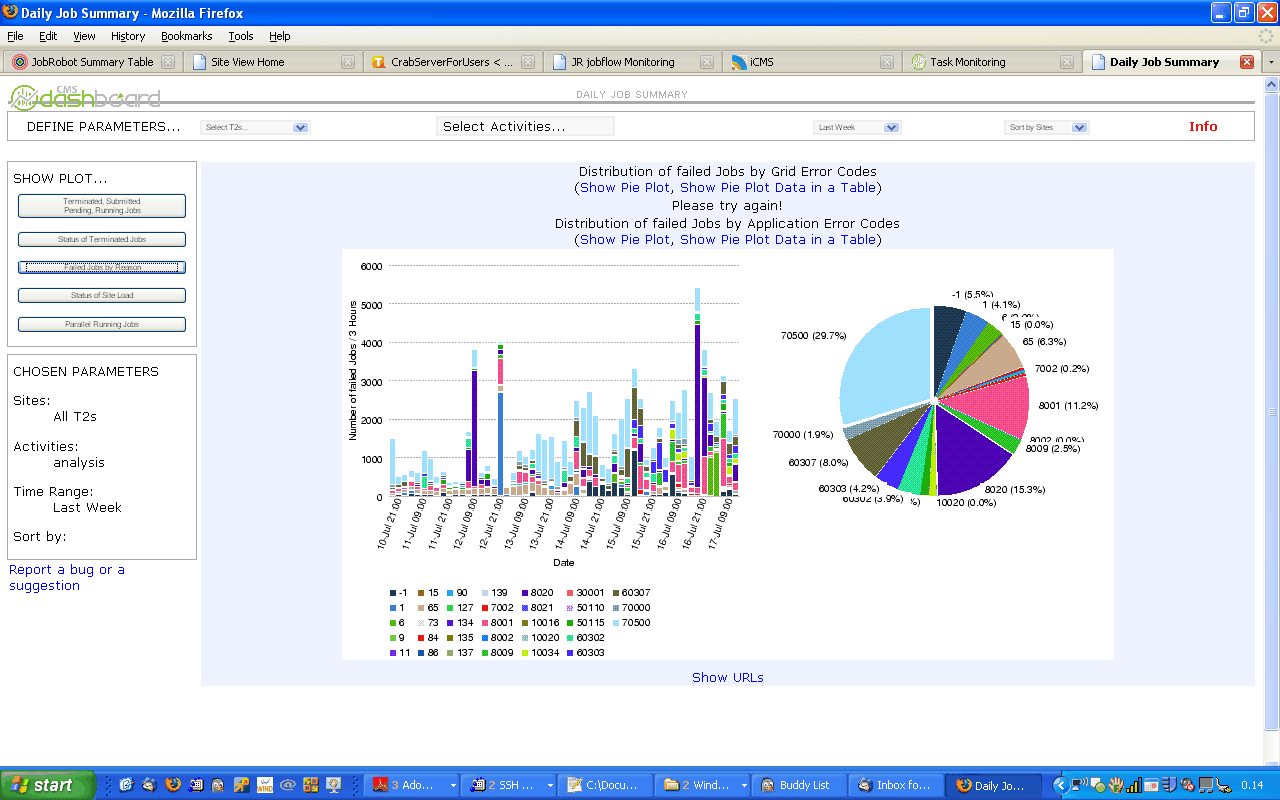
\includegraphics[width=0.70\textwidth]{figures/HistoryView.png}
\caption{All users tasks in last 2 days}
\label{fig:HistoryView}
\end{figure}
The list of viewable metrics is predefined, and
the interface uses aggregated tables in the DB to provide
efficient access to old information with a limited
amount of detail. Data can be viewed divided
according e.g. to the used site(s), job type or job completion status.


\subsection{Task Monitoring for Analysis user}
CRAB tasks usually have from a few hundred
to a thousand jobs each. A user will oftern submit one crab task
for each dataset used in a particular analysis, up to a few
tasks in one day. Task Monitoring for Analysis user was
developer as a user centric interface where the user is
initially presented the list of tasks he submitted in lasts
three days, both in tabular and graphical way (see Fig.~\ref{fig:TaskMonitor1}).

The user can then expand one selected task to get
a graphical overall summary of execution/completion progress
and access details of each job (see Fig.~\ref{fig:TaskMonitor2}).


\begin{figure}
 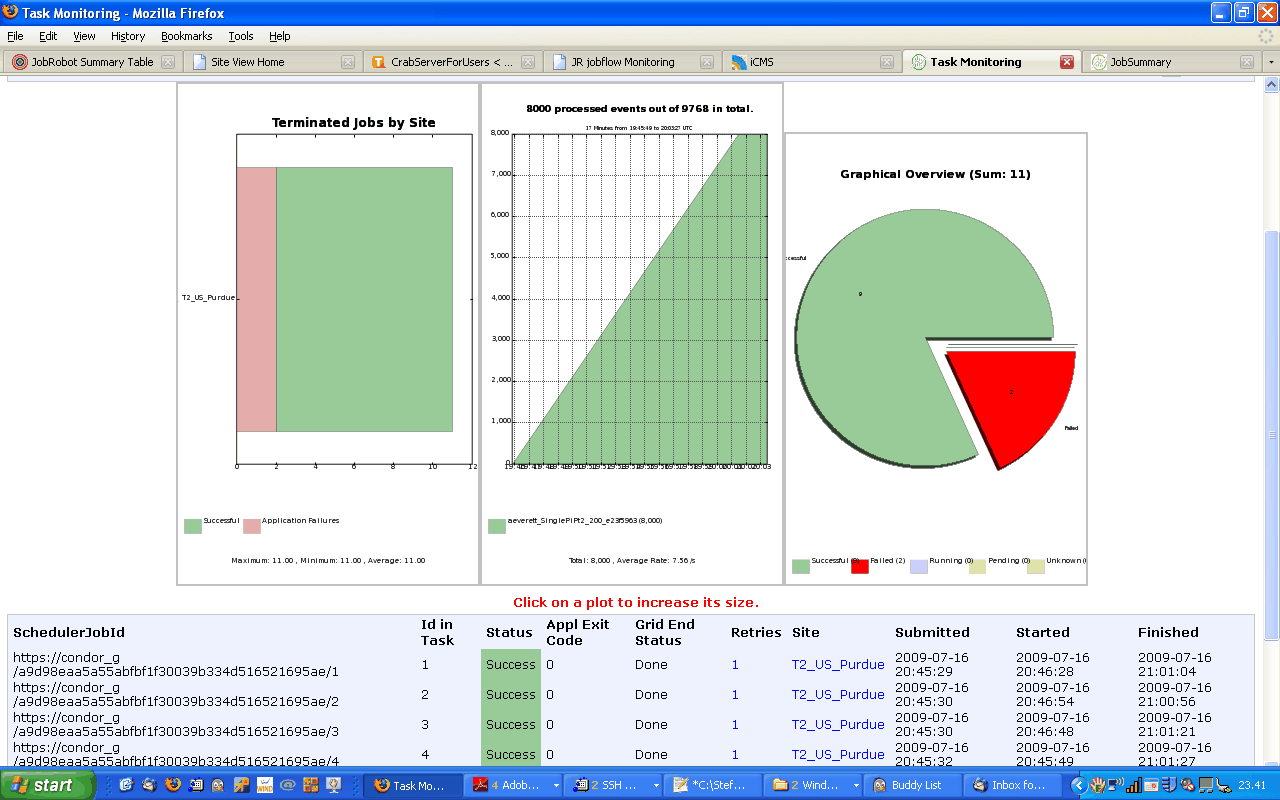
\includegraphics[width=0.50\textwidth]{figures/TaskMonitor1.png}
\caption{All users tasks in last 2 days}
\label{fig:TaskMonitor1}
\end{figure}
\begin{figure}
 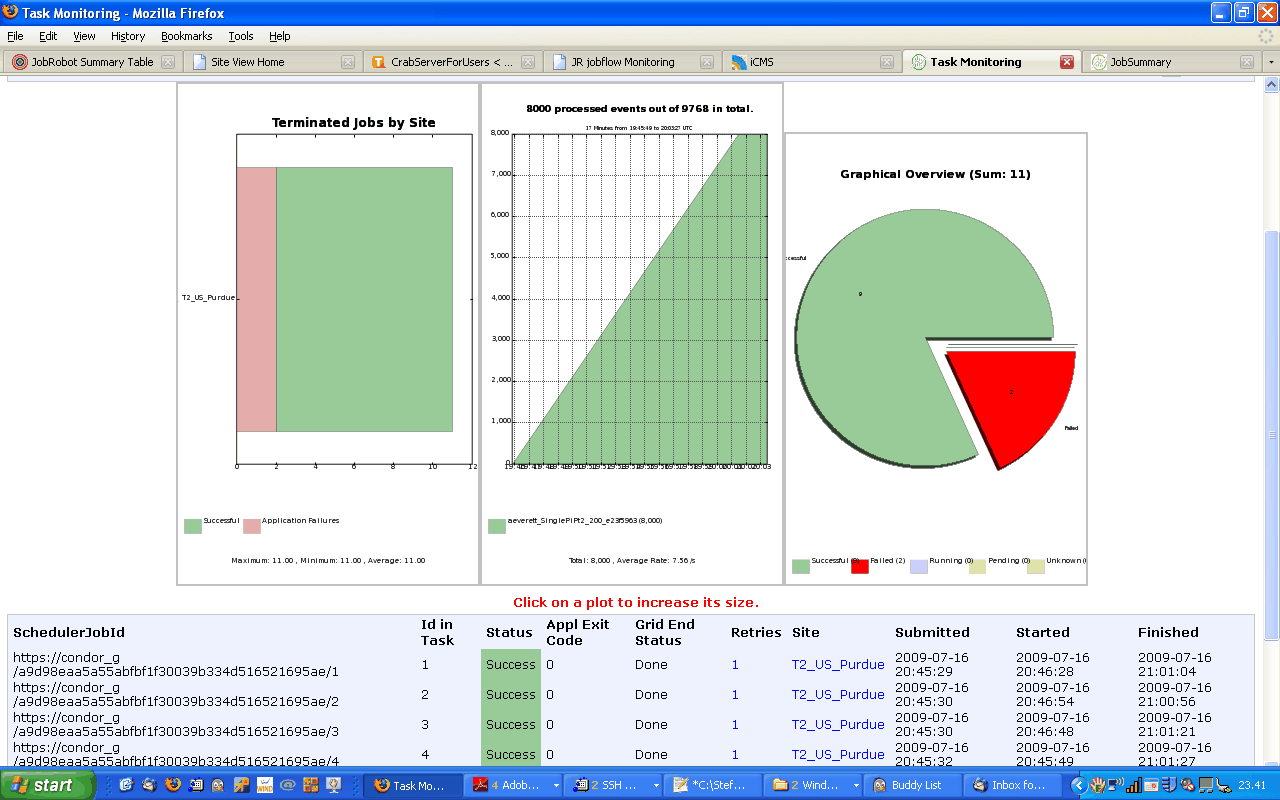
\includegraphics[width=0.50\textwidth]{figures/TaskMonitor2.png}
\caption{One task}
\label{fig:TaskMonitor2}
\end{figure}

\subsection{Interactive Interface}
Was the first view to be developed, based on
vision more then experience, therefore
emphasis was put on flexibility. It is a job-centric view
where the entry point is the number of jobs submitted or
terminated in a chosen time period (see Fig.~\ref{fig:Dashboard}).
\begin{figure}
 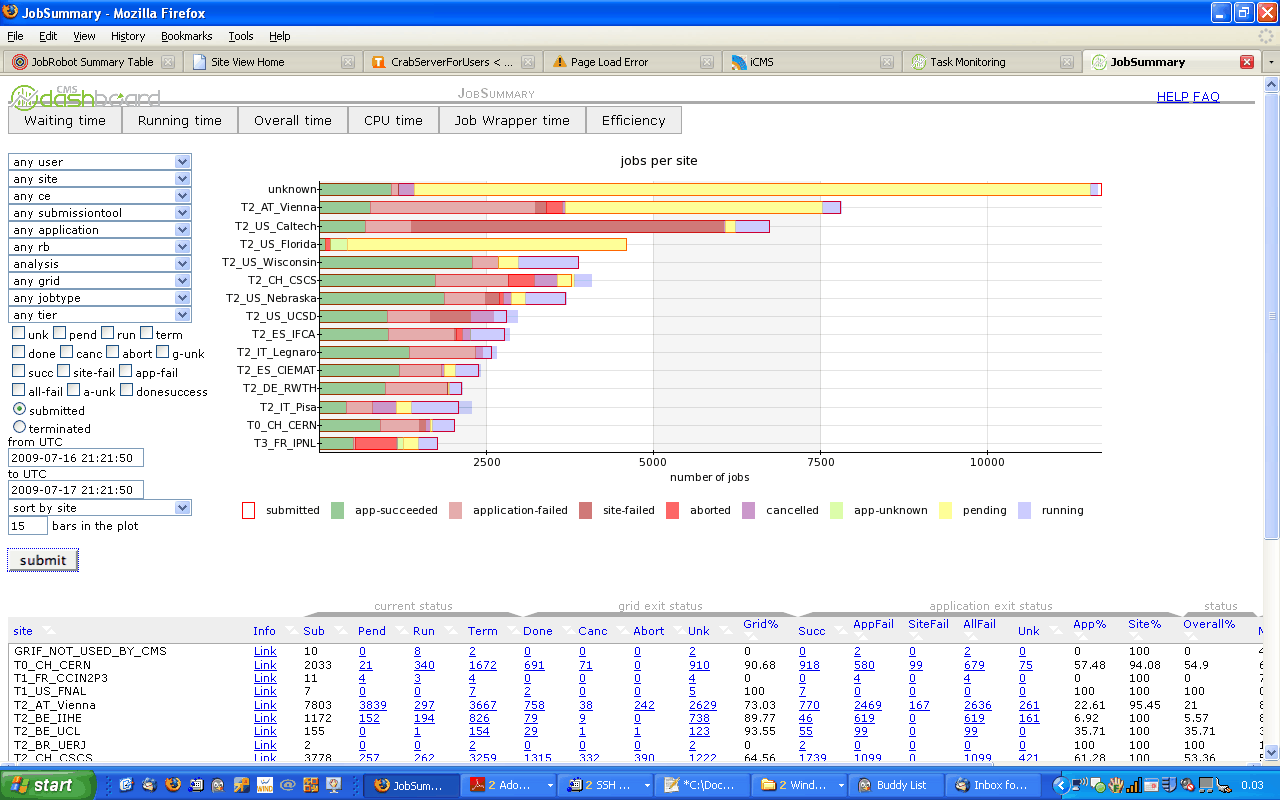
\includegraphics[width=0.80\textwidth]{figures/DashboardInteractive.png}
\caption{Dashboard Interactive Interface}
\label{fig:Dashboard}
\end{figure}
The interactive interface
allows to drill down expanding the set of jobs by
various relevant properties (execution site, grid gateway,
submitter user, completions status, grid workload management host,
activity type, used dataset etc.), until all details stored in the DataBase
about a choosen (set of) job(s) can be accessed.
The interface reports success/failure values and fractions
according to grid/site/application problem and information
on used wall and cpu time of jobs.
These kind of DataBase queries become more and more slow as the requested
time range expands, but details are only needed to analyse current issues.


